در این بخش، یک \lr{API} مبتنی بر \lr{GraphQL} برای سیستم مدیریت کارهای روزانه طراحی و پیاده‌سازی شده است. کاربران می‌توانند کار (\lr{Task}) بسازند، ویرایش یا حذف کنند، وضعیت را میان \lr{TODO}، \lr{DOING} و \lr{DONE} جابه‌جا کنند و کارها را با برچسب (\lr{Tag}) سازمان‌دهی کنند.

\subsubsection*{ استک فناوری و توجیه انتخاب}

\begin{itemize}
    \item {\lr{Node.js} و \lr{TypeScript}:} زبان و محیط اجرای پروژه؛ با توجه به اکوسیستم قوی \lr{GraphQL} در \lr{Node} انتخاب شد.
    \item {\lr{NestJS}:} فریم‌ورک ماژولار سمت سرور که تزریق وابستگی، ساختار لایه‌ای و یکپارچگی رسمی با \lr{GraphQL} را فراهم می‌کند.
    \item {\lr{Apollo Server}:} موتور اجرای \lr{GraphQL}؛ محیط تعاملی \lr{Apollo Sandbox} روی مسیر \lr{/graphql} برای کاوش اسکیم و تست عملیات در دسترس است.
    \item {\lr{@nestjs/graphql} با رویکرد \lr{Code-first}:} اسکیم از روی کلاس‌ها و \lr{decorator}های \lr{TypeScript} تولید می‌شود و فایل \lr{src/schema.gql} به‌صورت خودکار ساخته می‌شود؛ منبع حقیقت یکی است و \lr{type-safety} حفظ می‌شود.
    \item {\lr{Prisma} + \lr{SQLite}:} لایه دسترسی به داده با \lr{migration} و کلاینت تایپ‌شده؛ \lr{SQLite} پایگاه سبک و مناسب تمرین است و پشت پورت ریپازیتوری قابل تعویض با \lr{PostgreSQL} است.
    \item {\lr{class-validator} / \lr{class-transformer}:} اعتبارسنجی ورودی‌های \lr{Input} قبل از رسیدن به لایه دامنه.
    \item {\lr{DataLoader}:} حل مسئله کلاسیک \lr{N+1} برای فیلد رابطه‌ای \lr{Tag.tasks}.
    \item {\lr{graphql-depth-limit}:} محدود کردن عمق کوئری‌های تو در تو (حداکثر ۶) برای جلوگیری از سوءاستفاده.
    \item {\lr{nestjs-pino} / \lr{pino}:} لاگ ساختاریافته با شناسه همبستگی (\lr{request id}) و زمان اجرای هر عملیات \lr{GraphQL}.
    \item {\lr{Jest} + \lr{supertest}:} تست واحد (بدون دیتابیس) و تست \lr{e2e} روی اپ واقعی.
    \item {\lr{Docker} / \lr{docker-compose} و \lr{GitHub Actions}:} استقرار و اجرای خودکار \lr{CI} (لینت، بیلد، یونیت و \lr{e2e}).
\end{itemize}

\subsubsection*{معماری}

پروژه از {\lr{Clean Architecture}} پیروی می‌کند: وابستگی‌ها فقط به سمت داخل هستند و لایه دامنه هیچ وابستگی به \lr{NestJS}، \lr{Prisma} یا \lr{GraphQL} ندارد. هر ویژگی (\lr{tasks} و \lr{tags}) به چهار لایه تقسیم شده است:

\begin{enumerate}
    \item {\lr{domain}:} موجودیت‌ها، اینورینت‌ها، \lr{enum}ها، پورت ریپازیتوری (اینترفیس) و خطاهای دامنه‌ای.
    \item {\lr{application}:} یک \lr{Use Case} به‌ازای هر عملیات (مثلا \lr{CreateTask}، \lr{ListTasks}، \lr{UpdateTag}).
    \item {\lr{infrastructure}:} آداپتر \lr{Prisma} و \lr{mapper} تبدیل ردیف دیتابیس $\leftrightarrow$ موجودیت دامنه.
    \item {\lr{presentation}:} \lr{Object Type}ها، \lr{Input}ها، \lr{Resolver}ها و در صورت نیاز \lr{DataLoader}.
\end{enumerate}

مسیر یک درخواست به‌صورت خلاصه چنین است:
\begin{enumerate}
    \item دریافت درخواست \lr{POST /graphql}
    \item اعتبارسنجی اسکیم و عمق کوئری
    \item اعتبارسنجی ورودی با \lr{GqlValidationPipe}
    \item اجرای \lr{Resolver}
    \item فراخوانی \lr{Use Case}
    \item اعمال قوانین در موجودیت دامنه
    \item ذخیره/خواندن از طریق ریپازیتوری \lr{Prisma}
    \item دسترسی به \lr{SQLite}
\end{enumerate}

نکته طراحی مهم: فیلد \lr{Tag.tasks} داخل ماژول \lr{tasks} (\lr{TagTasksResolver}) پیاده شده تا وابستگی ماژول‌ها یک‌طرفه بماند (\lr{tasks} به \lr{tags}) و چرخه وابستگی ایجاد نشود.

\subsubsection*{ ساختار پوشه‌ها}

\begin{latin}
\begin{lstlisting}[language={},basicstyle=\ttfamily\footnotesize]
src/
  common/                 # config, errors, filters, pipes, pagination
  infrastructure/prisma/  # PrismaService
  health/                 # REST GET /health
  modules/
    tasks/{domain,application,infrastructure,presentation}
    tags/{domain,application,infrastructure,presentation}
  schema.gql              # auto-generated GraphQL schema
prisma/schema.prisma
postman/NestJS-GraphQL.postman_collection.json
test/                     # e2e
\end{lstlisting}
\end{latin}

\subsubsection*{ مدل داده}

دو موجودیت اصلی با رابطه چندبه‌چند وجود دارد:

\begin{itemize}
    \item {\lr{Task}:} عنوان اجباری، توضیحات اختیاری، وضعیت، اولویت، تاریخ سررسید، برچسب‌ها، \lr{createdAt} و \lr{updatedAt}.
    \item {\lr{Tag}:} نام یکتا، رنگ هگزادسیمال اختیاری، لیست کارهای مرتبط.
\end{itemize}

چون \lr{SQLite} در \lr{Prisma} از \lr{enum} بومی پشتیبانی نمی‌کند، وضعیت به‌صورت رشته و اولویت به‌صورت عدد صحیح (\lr{1=LOW} تا \lr{3=HIGH}) ذخیره می‌شود تا سورت اولویت معنادار باشد؛ ترجمه به \lr{enum} دامنه در \lr{mapper} انجام می‌شود.


\subsubsection*{کوئری‌ها}
\begin{itemize}
    \item \lr{tasks(filter, pagination, sort)} — فیلتر بر اساس وضعیت، اولویت، برچسب، جستجو در عنوان/توضیح و بازه سررسید؛ صفحه‌بندی \lr{skip/take} (حداکثر \lr{take=50})؛ مرتب‌سازی روی چند فیلد.
    \item \lr{task(id)} — در صورت نبودن، \lr{null} برمی‌گرداند.
    \item \lr{tags} و \lr{tag(id)}.
\end{itemize}

\subsubsection*{میوتیشن‌ها}
\begin{itemize}
    \item \lr{createTask} / \lr{updateTask} / \lr{deleteTask} / \lr{changeTaskStatus}
    \item \lr{createTag} / \lr{updateTag} / \lr{deleteTag}
\end{itemize}

\subsubsection*{ نکات پیاده‌سازی مهم}

\begin{itemize}
    \item {\lr{DataLoader} برای \lr{Tag.tasks}:} جلوگیری از \lr{N+1}؛ تمام \lr{tagId}های یک درخواست در یک کوئری دسته‌ای واکشی می‌شوند.
    \item {اعتبارسنجی ورودی:} محدودیت طول عنوان، فرمت رنگ، سقف صفحه‌بندی و غیره در لایه \lr{presentation}؛ قوانین کسب‌وکار (مثل عنوان خالی) در موجودیت دامنه.
    \item {سلامت سرویس:} مسیر \lr{REST} با آدرس \lr{/health} برای \lr{Docker healthcheck}.
    \item {تست:} بیش از ۶۰ تست واحد روی دامنه و \lr{use case}ها با ریپازیتوری درون‌حافظه‌ای، و بیش از ۲۰ تست \lr{e2e} روی دیتابیس موقت.
\end{itemize}

\subsubsection*{اجرا و نحوه تست}

\begin{latin}
\begin{lstlisting}[language={},basicstyle=\ttfamily\footnotesize]
cp .env.example .env
npx prisma migrate dev
npm run start:dev
# open http://localhost:3000/graphql  (Apollo Sandbox)
\end{lstlisting}
\end{latin}

برای پوشش کامل عملیات (ساخت/ویرایش/حذف کار و برچسب، تغییر وضعیت، فیلتر، سورت، صفحه‌بندی و نمونه‌های خطا) می‌توان از یکی از این دو روش استفاده کرد:
\begin{itemize}
    \item {\lr{Apollo Sandbox}:} اسکیم را در سمت چپ مرور کرده و کوئری/میوتیشن را با \lr{autocomplete} اجرا کنید.
    \item {کالکشن \lr{Postman}:} فایل \lr{postman/NestJS-GraphQL.postman\_collection.json} را ایمپورت کنید و پوشه‌ها را به ترتیب \lr{Health}، \lr{Tags}، \lr{Tasks} و \lr{Error examples} اجرا کنید. شناسه‌های ساخته‌شده در متغیرهای کالکشن ذخیره می‌شوند و درخواست‌های بعدی به‌صورت زنجیره‌ای کار می‌کنند.
\end{itemize}

\subsubsection*{نمونه‌های اجراشده}

در ادامه سه نمونه از عملیات اصلی برچسب‌ها که در \lr{Apollo Sandbox} اجرا شده‌اند آورده شده است. باقی درخواست‌ها (از جمله \lr{CRUD} کامل کارها، فیلتر، سورت و نمونه‌های خطا) از طریق همان \lr{Sandbox} یا کالکشن \lr{Postman} قابل تست هستند.

میوتیشن \lr{createTag} با نام \lr{random tag} و رنگ \lr{\#3366ff} اجرا شد و شناسه \lr{UUID} همراه با \lr{createdAt} برگردانده شد.

\begin{figure}[H]
\centering
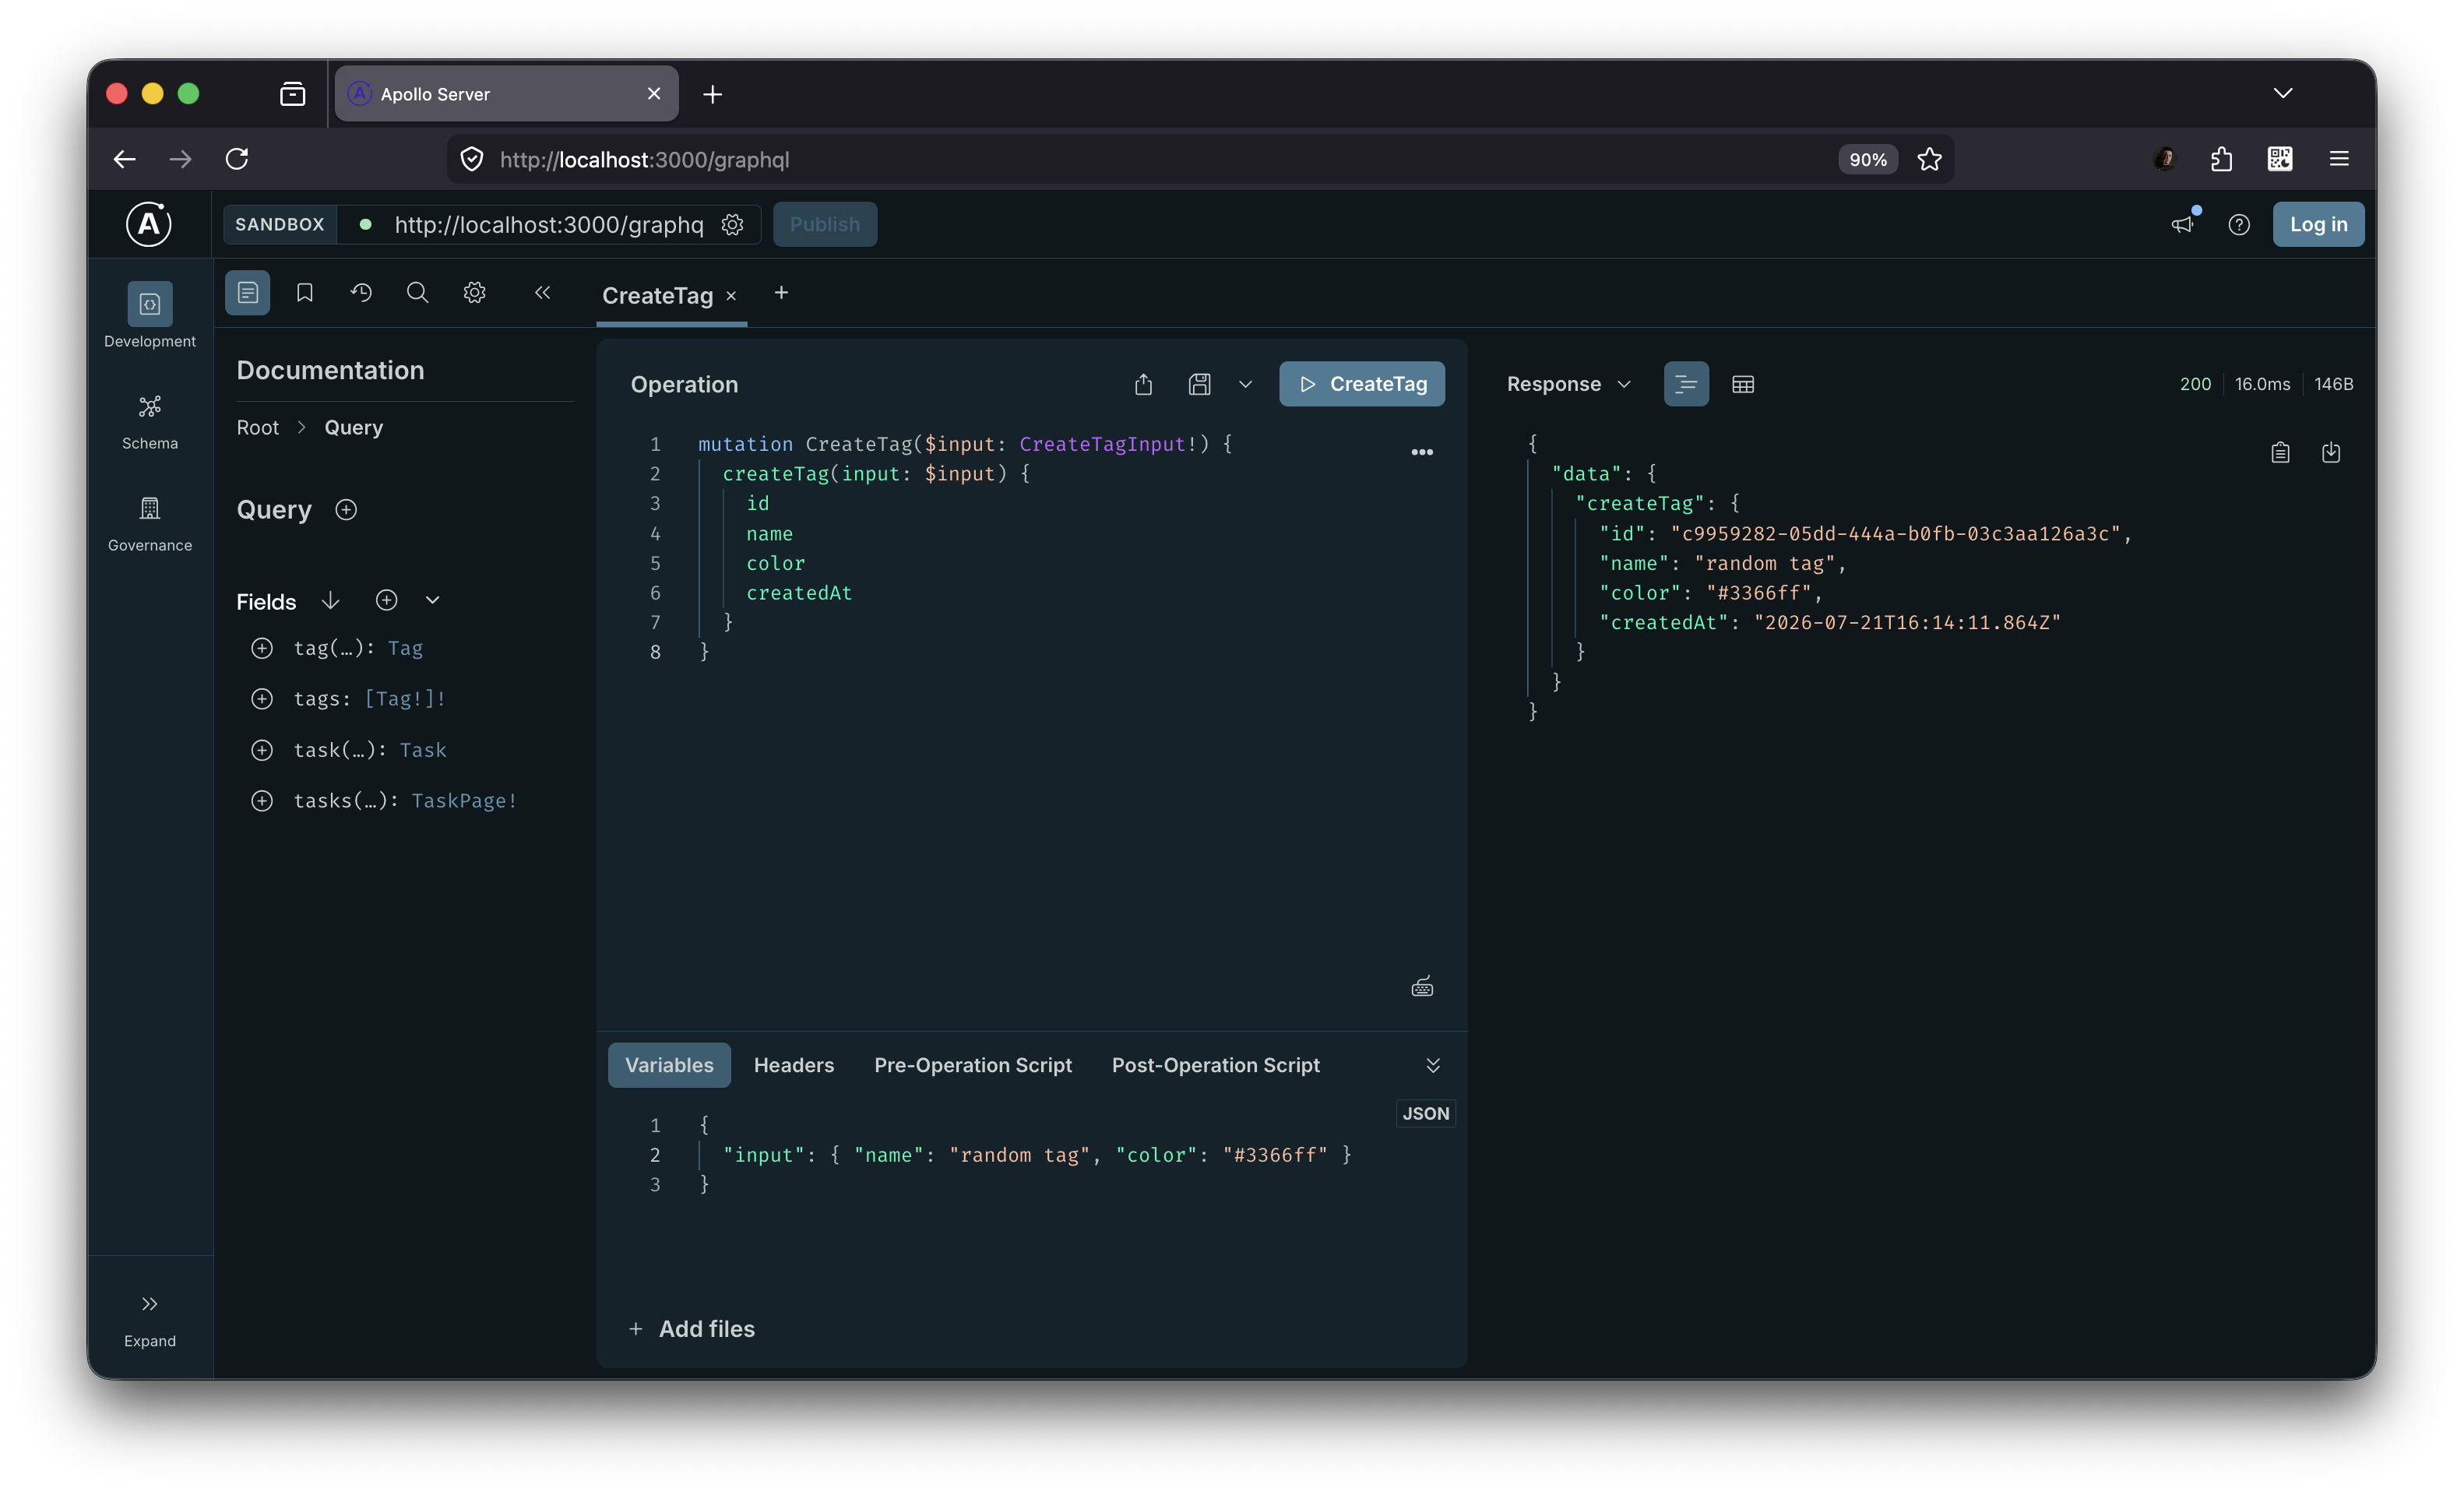
\includegraphics[width=0.7\textwidth]{figs/create-tag.png}
\end{figure}

کوئری \lr{tags} فیلدهای \lr{id}، \lr{name}، \lr{color} و رابطه تو در توی تسک‌ها (\lr{tasks} با فیلدهای \lr{id}، \lr{title} و \lr{status}) را درخواست می‌کند. این سناریو همان مسیری است که \lr{DataLoader} برای جلوگیری از \lr{N+1} به کار می‌آید.

\begin{figure}[H]
\centering
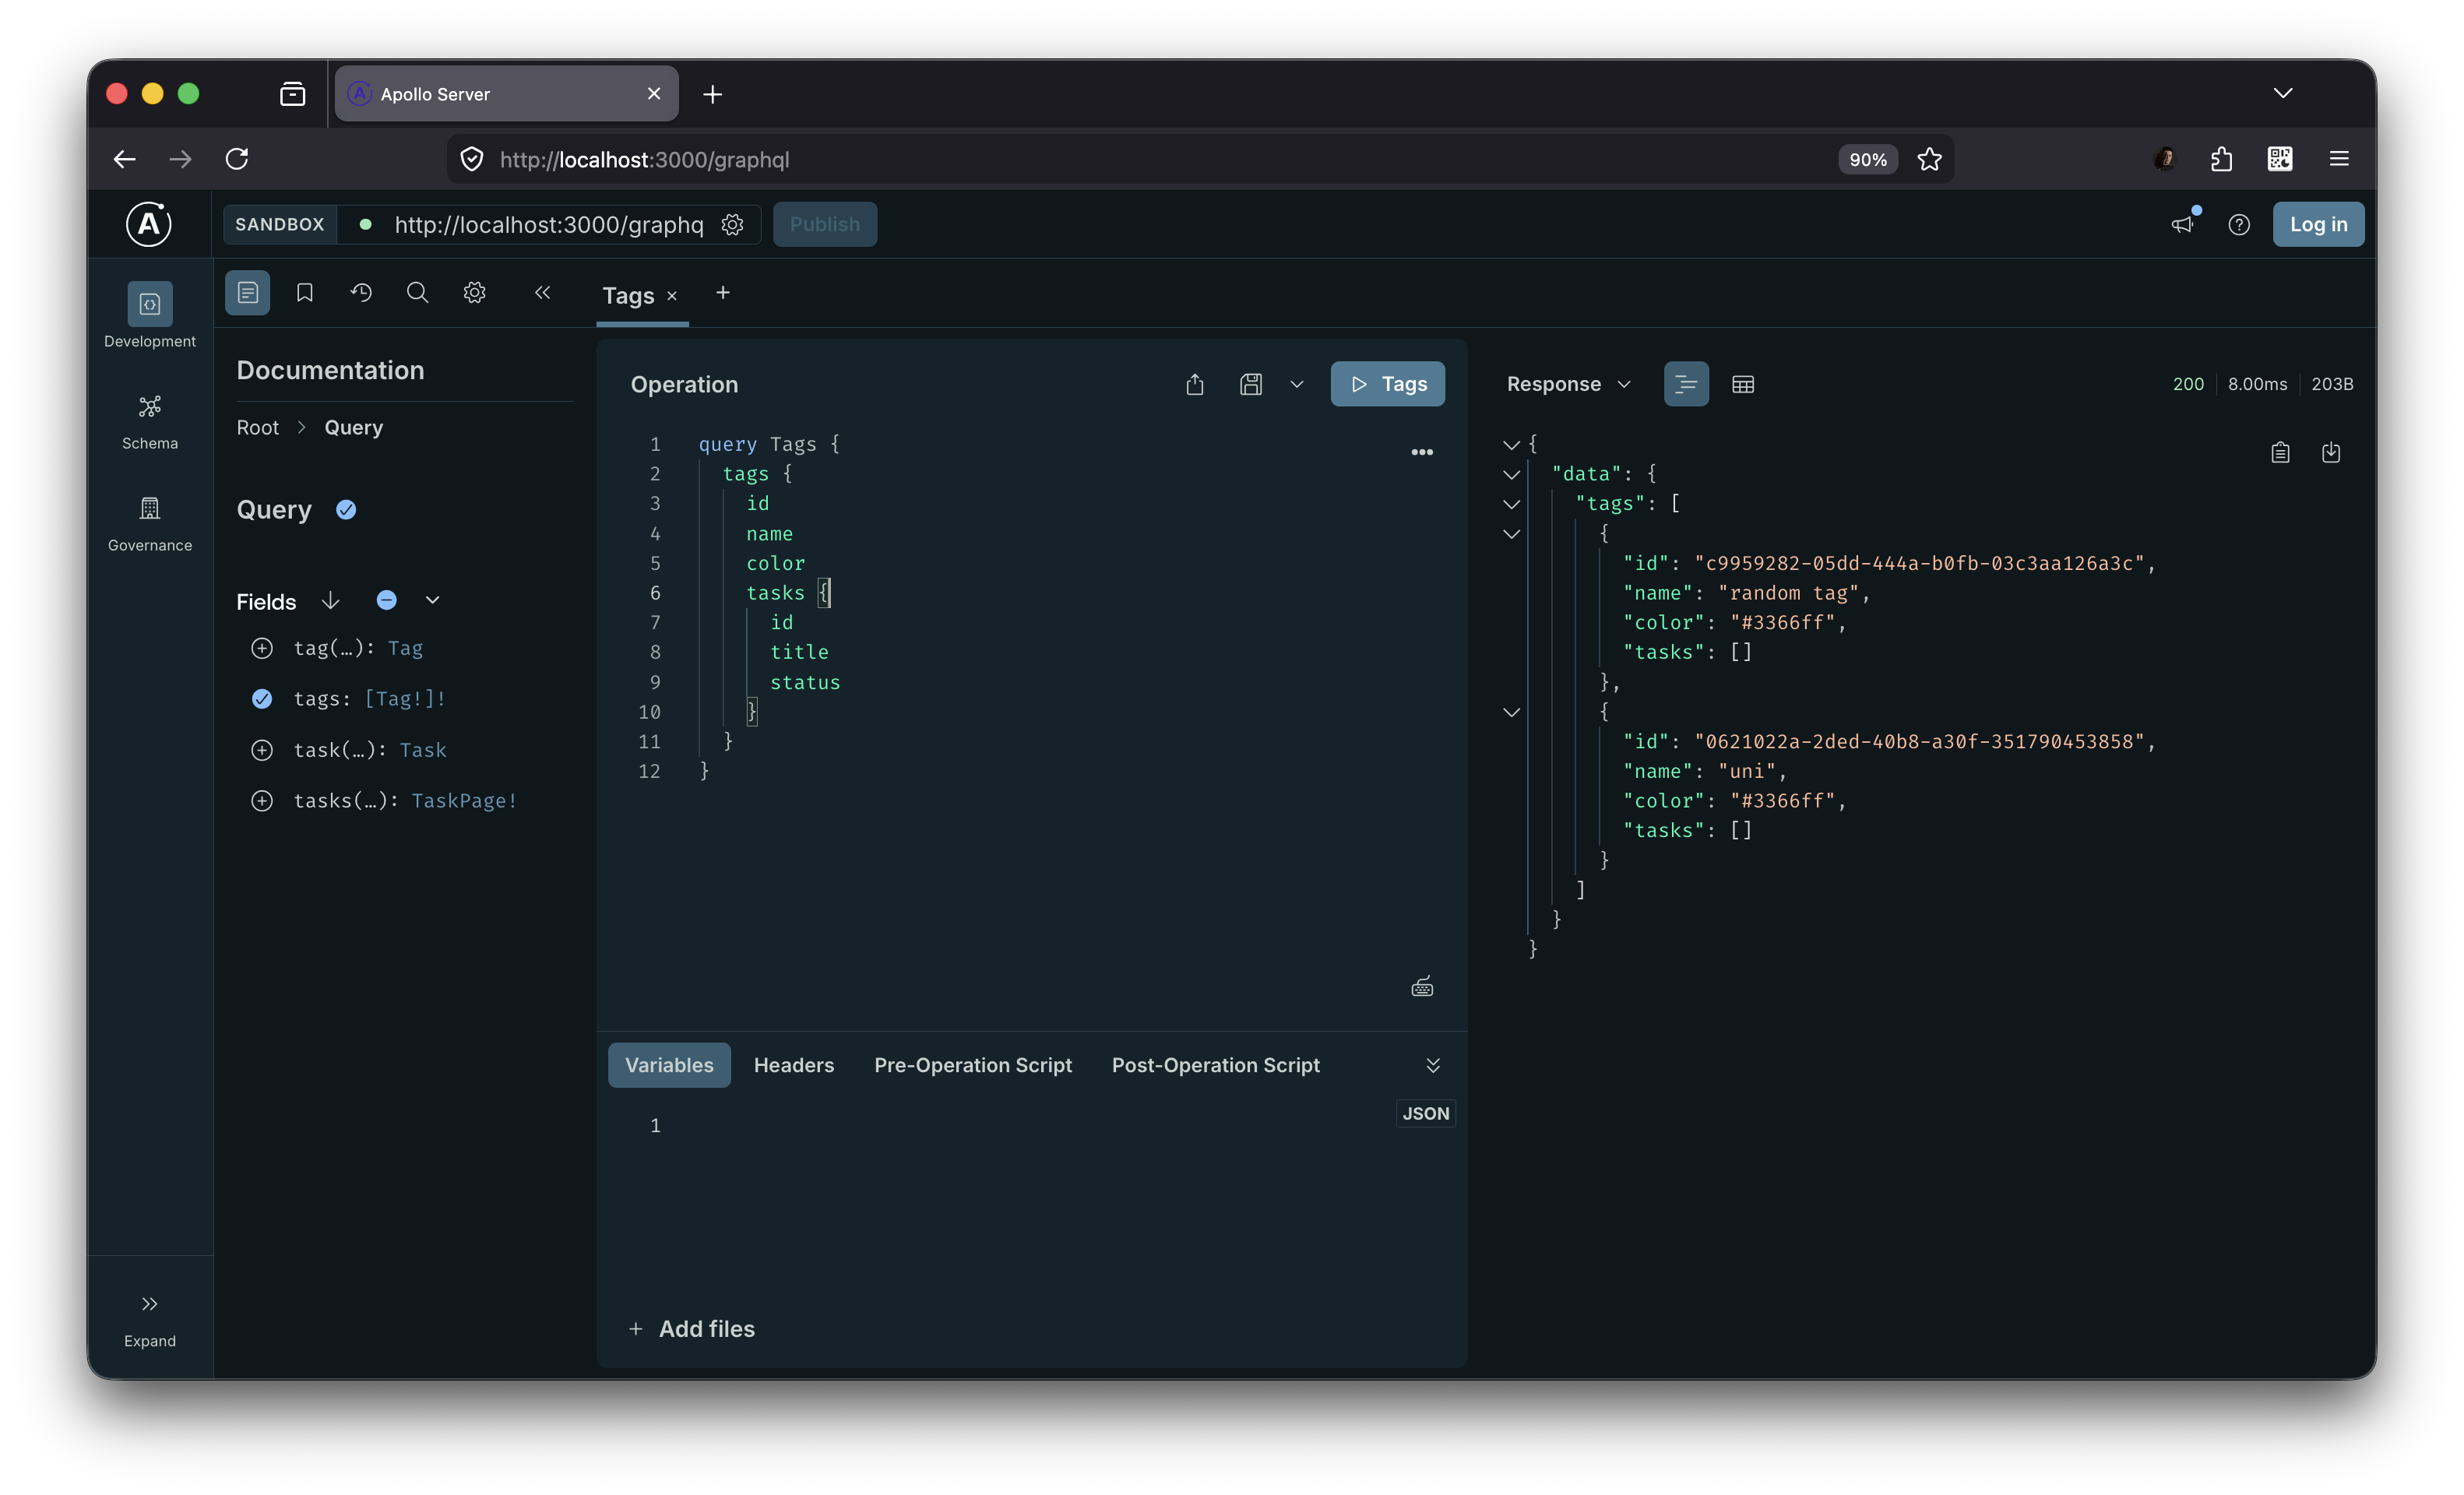
\includegraphics[width=0.7\textwidth]{figs/list-tags.png}
\end{figure}

میوتیشن \lr{updateTag} نام را به \lr{new random tag} و رنگ را به \lr{\#00aa55} تغییر داد و آبجکت به‌روزشده را برگرداند.

\begin{figure}[H]
\centering
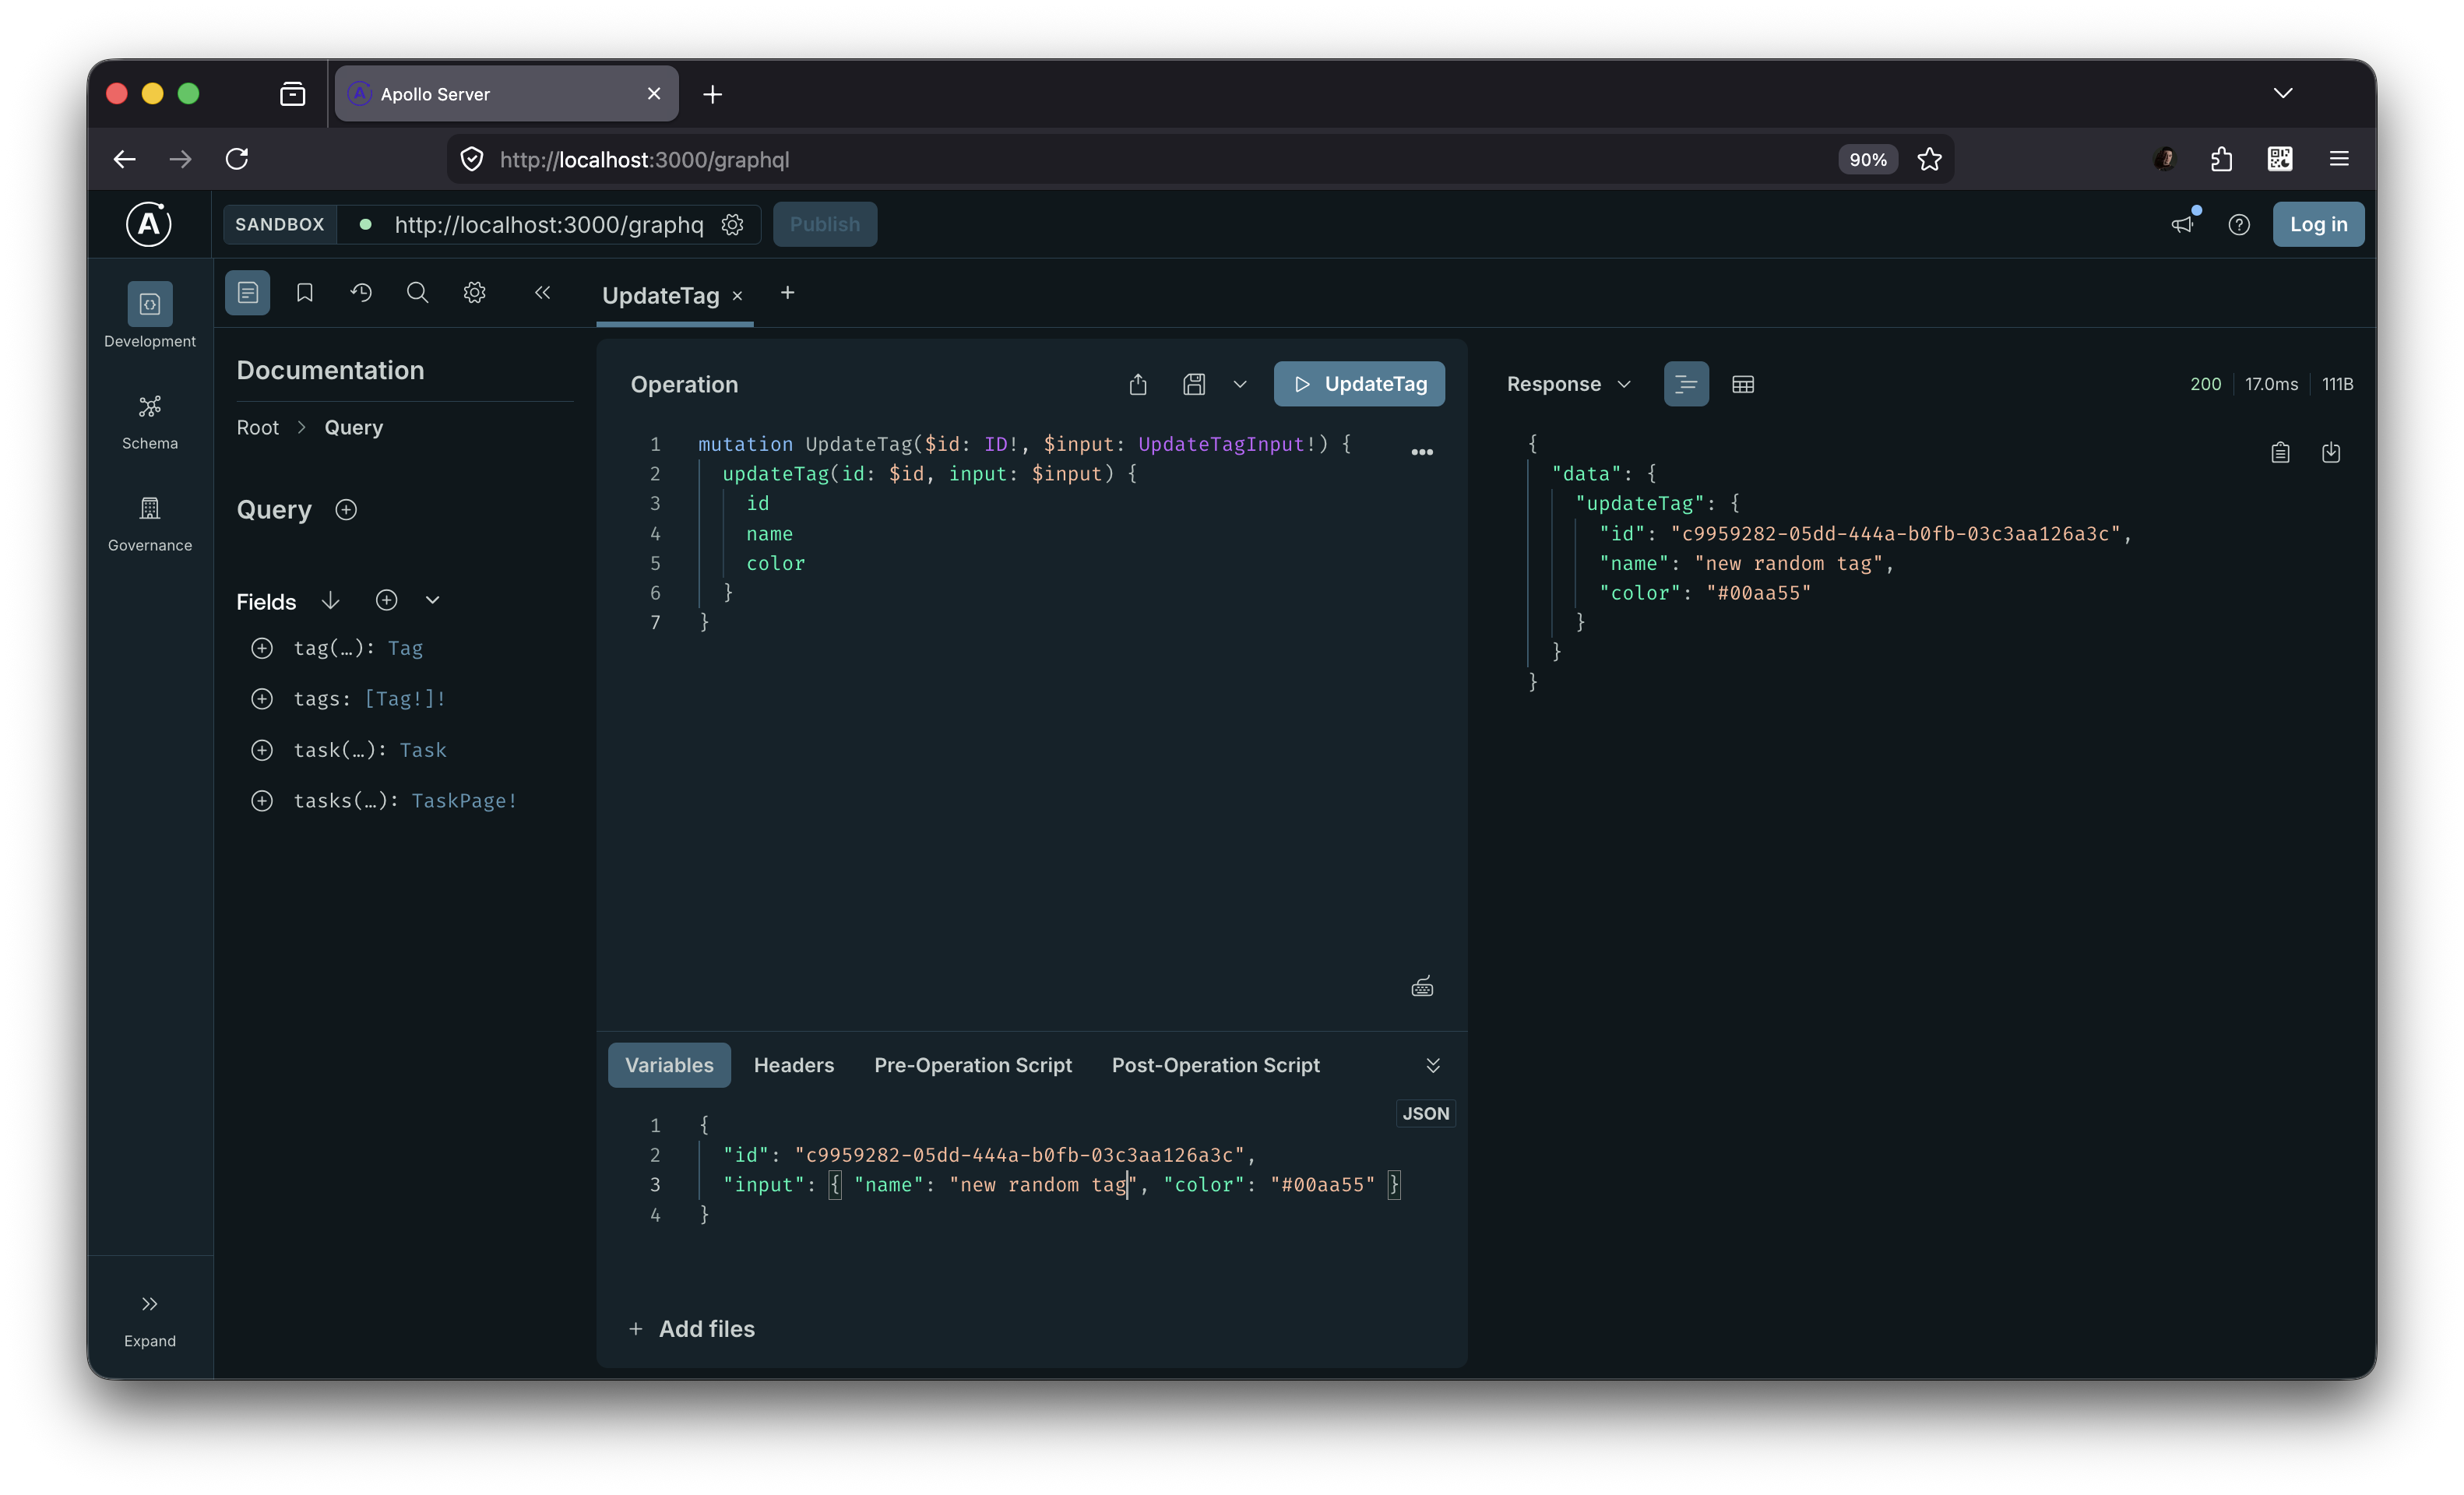
\includegraphics[width=0.7\textwidth]{figs/update-tag.png}
\end{figure}
